\section{Symmetry on Angular Correlation}
\subsection{Rotation of Data Points} \label{sec:PCA}
This section explains relation of rotation matrices and data points. It will be shown that redundancy or lowest number of independent parameter can be found by applying particular rotation matrix on data points.

Orthogonal transformation is a linear transformation that preserves the dot product of vectors. The length or radius of the vectors are not changed by applying an orthogonal transformation. Even more, the angle between two vectors are preserved. Applying orthogonal transformation on coordinate axes will result in rotation, reflection, or inversion of axes. Mathematically, an orthogonal transformation is represented as a rotation matrix. Basic theory about orthogonal transformations and rotation matrices is described in this section.   

\begin{figure}[h]
\begin{subfigure}{.5\textwidth}
  \centering
  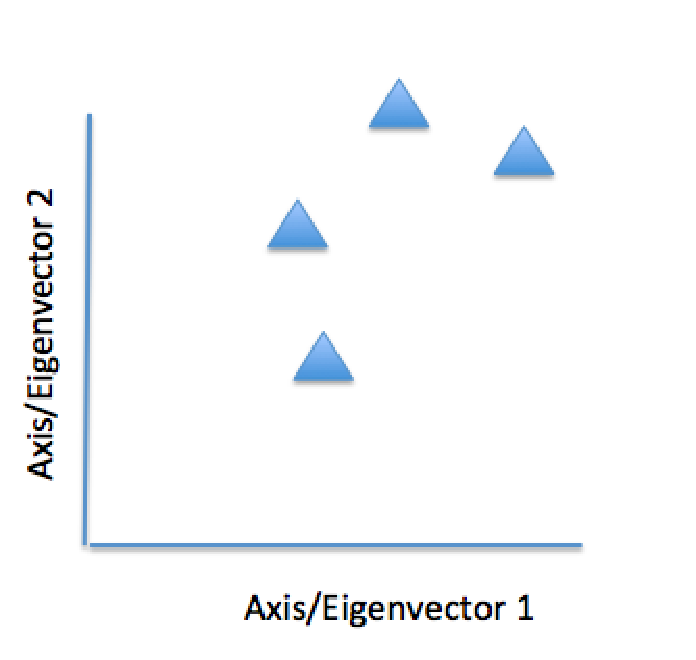
\includegraphics[width=.6\textwidth]{pointfree}
  \caption{Original axis}
\end{subfigure}
\begin{subfigure}{.5\textwidth}
  \centering
  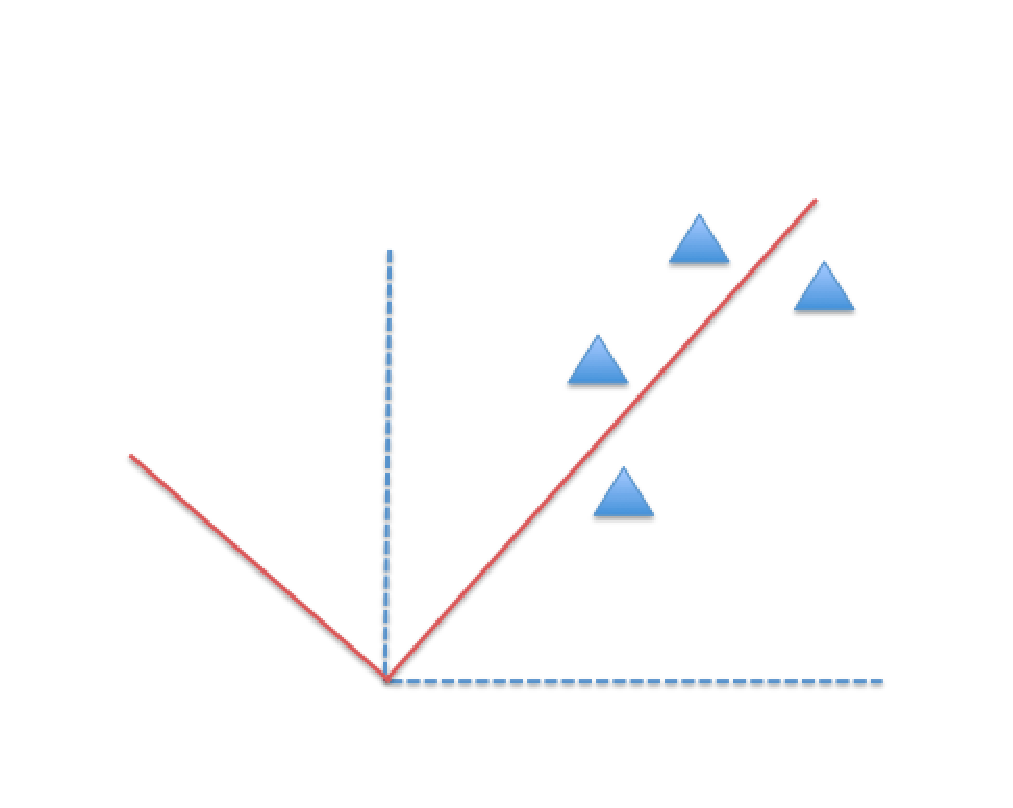
\includegraphics[width=.8\textwidth]{rotatedpoint}
  \caption{Rotated axis}
\end{subfigure}
\caption{Any point can be described in transformed axis}
\label{fig:rotatedaxis}
\end{figure}

Figure \ref{fig:rotatedaxis} illustrates that any point can be described in terms of any axes. As long as the relation of the new to the old axes is caused by an orthogonal transformation, the effect on data points is only rotation,  preserving radius or length of the data points. Throughout all rotation, there will be always an axis or direction in which one particular axis will have a smallest component as displayed in figure \ref{fig:axissmallercomponent},  By knowing that axis, it can be used to reduce the dimension of the data without losing essential information because axis with the smallest component has the least information.    



\begin{figure}[h]
  \centering
  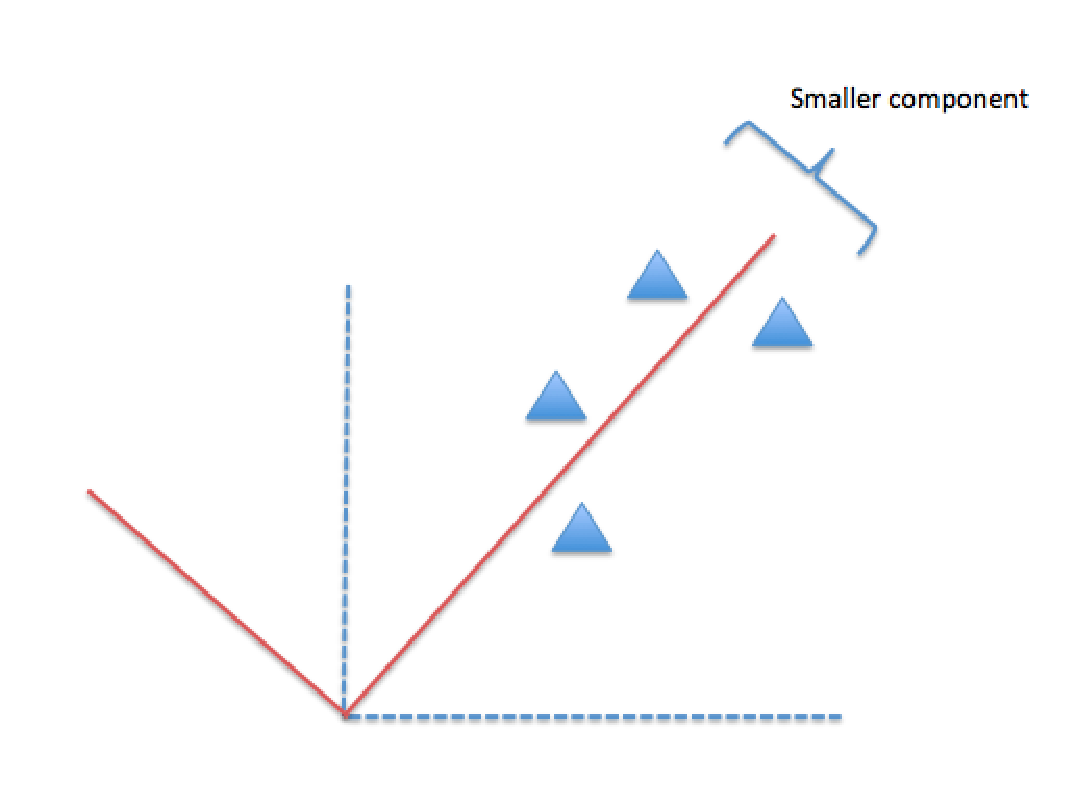
\includegraphics[width=.8\textwidth]{rotatedpointsmaller}
\caption{Red is axis in which has maximum variance in one direction and minimum component in another one}
\label{fig:axissmallercomponent}
\end{figure}

\begin{figure}[h]
  \centering
  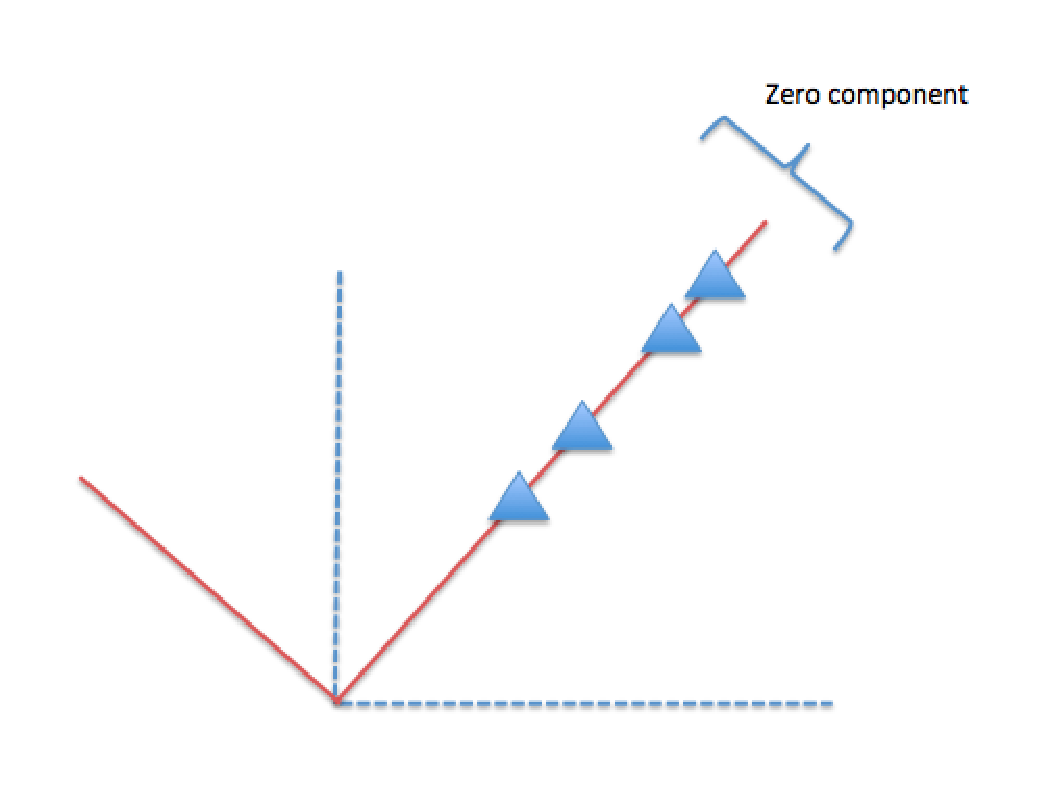
\includegraphics[width=.8\textwidth]{rotatedpointzero}
\caption{In red axis, data can be specified with one parameter only}
\label{fig:axisoneparameter}
\end{figure}
A rotation matrix can be used to indicate whether there is redundant information in data set. A redundancy means there is a different way to represent data with a lower number of independent parameters. Illustrated in figure \ref{fig:axisoneparameter}, the data points are represented by two different ways, using blue axes the data are specified using two parameters whereas using the red axis the data are specified with one parameter. If the data contain redundant information, then the number of independent parameters can be reduced by rotating the axes. Figure \ref{fig:axisoneparameter} shows that redundancy in 2D occurs due to the data lying in the same line. Generalizing into higher dimension, the redundancy occur  when the data lie in either a line, a plane, or a hyperplane. 

Essential property to find the lowest number of independent parameter is knowing that the dot product between the  data set is enough to reveal the redundancies.  From figure \ref{fig:axisoneparameter}, all data point have the same angle from each other. Since the angle is obtainable from the dot product, by constructing a matrix of dot products, a pattern appear whether there is a redundancy inside data sets. The redundancy in 2D case is very simple; if the angle is the same for the all data set, then there is redundancy. To reveal the redundancy in higher order, a different sophisticated method is needed, because a common pattern in dot product is not easily observable. 

One of the method to reveal redundancy of the data in higher dimension is the principal component analysis. The next section will explain the principal component analysis and how it can be used to determine symmetry of particles only from correlation data.  

\subsection{Principal Component  Analysis }
Principal component analysis (PCA) is an established method to reduce the dimension of a set of vectors. PCA uses orthogonal transformation to convert a set of vectors into a set of new vectors. The determination of the orthogonal transformation is defined in such a way that one axis will have the largest variance and another axis will have the smallest component. In addition to that, PCA can be used to find the lowest number of independent parameters in a data set, which is the purpose of this section. 

Another important point is that the rotation of an axis can be used to find the lowest number of independent parameters in the data set. A set of vectors in any arbitrary independent axis can be described as
\begin{eqnarray}
\vec{V_{1}}=
\begin{bmatrix}
\upsilon_{11}&\upsilon_{12} & \ldots & \upsilon_{1m}
\end{bmatrix}\\ \nonumber
\vec{V_{2}}=
\begin{bmatrix}
\upsilon_{21}&\upsilon_{22} & \ldots & \upsilon_{2m}
\end{bmatrix}\\ \nonumber
\vec{V_{3}}=
\begin{bmatrix}
\upsilon_{31}&\upsilon_{32} & \ldots & \upsilon_{3m}
\end{bmatrix}\\ \nonumber
\vec{V_{n}}=
\begin{bmatrix}
\upsilon_{n1}&\upsilon_{n2} & \ldots & \upsilon_{nm}
\end{bmatrix}\\ \nonumber
.
\end{eqnarray}
To represent this set of vectors as a set of new data, a matrix can be formed by arranging each row as new independent vectors and each column as an independent components. The matrix is  
\begin{eqnarray}
\mathbf{V}=
\begin{bmatrix}
\upsilon_{11}&\upsilon_{12} & \ldots & \upsilon_{1m} \\
\upsilon_{21}&\upsilon_{22} & \ldots & \upsilon_{2m} \\
\upsilon_{31}&\upsilon_{32} & \ldots & \upsilon_{3m} \\
\vdots & \vdots \\
\upsilon_{n1}&\upsilon_{n2} & \ldots & \upsilon_{nm} 
\end{bmatrix}.
\end{eqnarray} 
From that new definition, a new quantity called covariance matrix is defined as
\begin{eqnarray}
\mathbf{C}=\mathbf{V^{t}}\mathbf{V}.
\end{eqnarray} 

Based on PCA, the first eigenvector of the covariance matrix is the direction of the maximum variance or the minimum residual component. In addition to that, finding the lowest independent parameters to describe the system can be found from counting the nonzero eigenvalues of the covariance matrix. In addition to that, calculating eigenvectors and eigenvalues can be done by using singular value decomposition (SVD). Mathematically, the SVD is 

\begin{eqnarray}
[u \, s \, v ]=\mbox{SVD}(\mathbf{V^{t}}\mathbf{V})
\end{eqnarray} 
where $u$ is a matrix composed of independent eigenvectors and $s$ is a matrix consist of eigenvalues of covariance matrix. 

Neither $\mathbf{V^{t}}\mathbf{V}$ nor $\mathbf{V}$ are available from the angular correlation data. Only the matrix of dot product is available. It will be shown below that matrix of dot product will have eigenvalues equal to the eigenvalues of covariance matrix. 

The matrix of the dot product is defined as
\begin{eqnarray}
\mathbf{M_{d}} &=& 
\begin{bmatrix}
\vec{V_{1}}\cdot\vec{V_{1}} &\vec{V_{1}}\cdot\vec{V_{2}} & \ldots & \vec{V_{1}}\cdot\vec{V_{m}} \\
\vec{V_{2}}\cdot\vec{V_{1}} &\vec{V_{2}}\cdot\vec{V_{2}} & \ldots & \vec{V_{2}}\cdot\vec{V_{m}} \\
\vec{V_{3}}\cdot\vec{V_{1}} &\vec{V_{3}}\cdot\vec{V_{2}} & \ldots & \vec{V_{3}}\cdot\vec{V_{m}} \\
\vdots & \vdots \\
\vec{V_{n}}\cdot\vec{V_{1}} &\vec{V_{n}}\cdot\vec{V_{2}} & \ldots & \vec{V_{n}}\cdot\vec{V_{m}} \\
\end{bmatrix}
\\
&=& \vec{V} \vec{V^{t}}.
\end{eqnarray}
Having defined the matrix of the dot product, its eigenvalue can be found from the covarianve matrix or covariance matrix's eigenvalue can be found from the matrix of the dot product. The proof is shown below: 
\begin{eqnarray}
\mathbf{M_{d}} \, \nu &=& \lambda \, \nu \\ \nonumber
\vec{V} \, \vec{V^{t}} \, \nu &=& \lambda \, \nu \\ \nonumber
%\mbox{left multiplication with } \vec{V^{t}} \mbox{yield}  \\
\vec{V^{t}} \, \vec{V} \, \vec{V^{t}} \, \nu &=& \lambda \, \vec{V^{t}}\, \nu \\ \nonumber
\vec{V^{t}} \, \vec{V} \, \mu &=& \lambda \, \mu 
\label{eq:matrixofdotproduct}
\end{eqnarray}

In conclusion, $\vec{V} \, \vec{V^{t}}$ and $\vec{V^{t}} \, \vec{V}$ have equal eigenvalues but different eigenvectors. The eigenvalue that give the lowest independent component is the eigenvalue of the covariance matrix. Hence, the eigenvalue of the covariance matrix can be easily be calculated by finding the eigenvalue of matrix of dot product. 

\subsection{Matrix Correlation}
As described in section \ref{sec:angcor}, the final expression obtained from the correlation data is
\begin{eqnarray}
B_{l}(q,q')=\sum_{m} I_{lm}(q) I_{lm}(q')^{*}. 
\end{eqnarray}
It is important to note that \Blq is a form of dot product depending of how one constructs vectors from $I_{lm}(q)$. Since every $I_{lm}(q)$ comes from spherical harmonics decomposition, every element is independent. A set of new vectors can be constructed where the value $m$'s correspond to the components and $q$'s correspond to the vectors for all $l$'s. As an example, the vectors constructed from this definition are
\begin{eqnarray}
I_{l}(q_1)=
\begin{bmatrix}
I_{l(-l)}(q_1)&I_{l(-l+1)}(q_1) & \ldots &I_{l(l)}(q_1)
\end{bmatrix}\\ \nonumber
I_{l}(q_2)=
\begin{bmatrix}
I_{l(-l)}(q_2)&I_{l(-l+1)}(q_2) & \ldots &I_{l(l)}(q_2)
\end{bmatrix}\\ \nonumber
I_{l}(q_3)=
\begin{bmatrix}
I_{l(-l)}(q_3)&I_{l(-l+1)}(q_3) & \ldots &I_{l(l)}(q_3)
\end{bmatrix}\\ \nonumber
I_{l}(q_n)=
\begin{bmatrix}
I_{l(-l)}(q_n)&I_{l(-l+1)}(q_n) & \ldots &I_{l(l)}(q_n)
\end{bmatrix}.\\ \nonumber
\end{eqnarray}
The expression $\sum_{m} I_{lm}(q) I_{lm}(q')^{*}$ is equivalent to $ \langle I_{l}(q) , I_{l}(q') \rangle$ that is the dot product of $I_{l}(q)$. Now with that definition, \Blq is a dot product of vectors $I_{lm}(q)$. 

After confirming that \Blq is the dot product of the vector \Ilm, a new matrix must be constructed in order to be used in PCA. There are infinite possible ways to construct a matrix from a set of vectors. In order to be used in PCA, the matrix of dot products is constructed by arranging all possible dot products of different vectors or $q$ points. Below is how matrix is constructed
\begin{eqnarray}
\mathbf{B_{qq'}^{l}} &=& 
\begin{bmatrix}
\langle I_{l}(q_1), I_{l}(q_1)\rangle & \langle I_{l}(q_1),I_{l}(q_2) \rangle & \ldots & \langle I_{l}(q_1),I_{l}(q_m) \rangle \\
& & \\
\langle I_{l}(q_2), I_{l}(q_1)\rangle & \langle I_{l}(q_2),I_{l}(q_2) \rangle & \ldots & \langle I_{l}(q_2),I_{l}(q_m) \rangle \\
& &\\
\langle I_{l}(q_3), I_{l}(q_1)\rangle & \langle I_{l}(q_3),I_{l}(q_2) \rangle & \ldots & \langle I_{l}(q_3),I_{l}(q_m) \rangle \\
\vdots & \vdots & \vdots \\
\langle I_{l}(q_n), I_{l}(q_1)\rangle & \langle I_{l}(q_n),I_{l}(q_2) \rangle & \ldots & \langle I_{l}(q_n),I_{l}(q_m) \rangle \\
\end{bmatrix}
\\
&=&
\begin{bmatrix}
B_{l}(q_1,q_1) &B_{l}(q_1,q_2)& \ldots& B_{l}(q_1,q_m) \\
& & \\
B_{l}(q_2,q_1) &B_{l}(q_2,q_2)& \ldots& B_{l}(q_2,q_m) \\
& &\\
B_{l}(q_3,q_1) &B_{l}(q_3,q_2)& \ldots& B_{l}(q_3,q_m) \\
\vdots & \vdots & \vdots \\
B_{l}(q_n,q_1) &B_{l}(q_n,q_2)& \ldots& B_{l}(q_n,q_m) \\
\end{bmatrix}
\end{eqnarray}

All elements of matrix $\mathbf{B_{qq'}}$ are obtainable from experiment according to eq \ref{eq:theB}. The matrix satisfies requirement to be a matrix of dot product as given in eq. \ref{eq:matrixofdotproduct}. The singular values of the matrix contain the information about the redundancy of the data. By counting how many nonzero singular value, those number can be used to describe the redundancy in vector $I_{lm}(q)$. 

The number of significant nonzero singular values represent total parameter to describe the data. Only nonzero singular value contribute to the independent parameters. The nonsignificant or zero singular values denote the number of redundant parameters. By comparing how many significant or nonzero, nonsignificant or zero, and total singular values, those information later is essential to predict the symmetry of the particle. 
%\end{document}
